\section{Scalar-Valued Functions of Several Variables}

\begin{definition}{Scalar Function}{scalar_function}
A scalar-valued function of several variables maps a vector of multiple inputs to a single real output $f: D \subseteq \mathbb{R}^n \to \mathbb{R}$.
\end{definition}

\textbf{Examples:}
\begin{itemize}
    \item Temperature distribution: $T(\text{longitude}, \text{latitude}, \text{time}): \mathbb{R}^3 \to \mathbb{R}$.
    \item Precipitation depth: $P(\text{longitude}, \text{latitude}): \mathbb{R}^2 \to \mathbb{R}$.
    \item Domain and Range example: For $f(x, y) = y\sqrt{x - 1}$,
    \[
    \text{Domain: } \{(x, y) \in \mathbb{R}^2 : x \geq 1\}, \quad \text{Range: } \mathbb{R}
    \]
\end{itemize}

\subsection{Visualizing Multivariable Functions: Traces and Level Sets}

The graph of a function $f(x, y)$ is defined as the surface $\{(x, y, z) \in \mathbb{R}^3 : z = f(x, y)\}$.

\begin{example}[Analyzing Traces of $f(x,y) = y\sin x$]
To visualize $f(x, y) = y \sin x$, we examine slices along constant coordinates (traces):

\begin{itemize}
    \item \textbf{$y$-traces ($y = c$):} \\
    For $y = 0 \implies z = 0$; \\
    for $y = 1 \implies z = \sin x$; \\
    for $y = -1 \implies z = -\sin x$. (Sinusoidal curves scaled by $y$). 
    \item \textbf{$x$-traces ($x = c$):} \\
    For $x = 0 \implies z = 0$; \\
    for $x = \frac{\pi}{2} \implies z = y$; \\
    for $x = \pi \implies z = 0$. (Lines whose slopes depend on $\sin x$). 
\end{itemize}
\end{example}

\subsection{Level Sets and Contour Maps}

\begin{definition}{Level Set}{level_set}
For a function $f: D \to \mathbb{R}$ ($D \subseteq \mathbb{R}^2$), the \textbf{level set} (or level curve) at height $c$ is defined as
\[
\{(x, y) \in \mathbb{R}^2 : f(x, y) = c\}.
\]
A collection of such level curves forms a \textbf{contour map}.
\end{definition}
\begin{example}[Comparing Level Curves]
Consider three functions and their level sets $f(x,y) = c$:
\begin{enumerate}
    \item $f(x, y) = \sqrt{x^2 + y^2}$: Level sets are equally spaced concentric circles $x^2 + y^2 = c^2$ (a cone).
    \item $g(x, y) = x^2 + y^2$: Level sets are circles $x^2 + y^2 = c$ spaced closer together as $c$ increases (a paraboloid).
    \item $h(x, y) = (x^2 + y^2)^{1/3}$: Level sets are circles $x^2 + y^2 = c^3$ spaced further apart as $c$ increases.
\end{enumerate}
\end{example}

\begin{figure}[htbp]
\centering
\begin{minipage}[t]{0.32\textwidth}
\centering
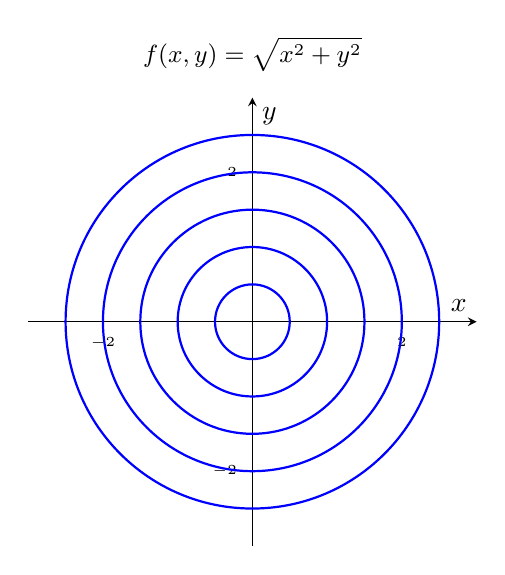
\begin{tikzpicture}
\begin{axis}[
    title={$f(x,y)=\sqrt{x^2+y^2}$},
    xlabel=$x$, ylabel=$y$,
    xmin=-3, xmax=3, ymin=-3, ymax=3,
    axis lines=middle,
    axis equal image,
    tick label style={font=\tiny},
    title style={font=\small}
]
    \pgfplotsinvokeforeach{0.5, 1.0, 1.5, 2.0, 2.5}{
        \draw[blue, thick] (axis cs:0,0) circle [radius=#1)];
    }
\end{axis}
\end{tikzpicture}
\end{minipage}
\hfill
\begin{minipage}[t]{0.32\textwidth}
\centering
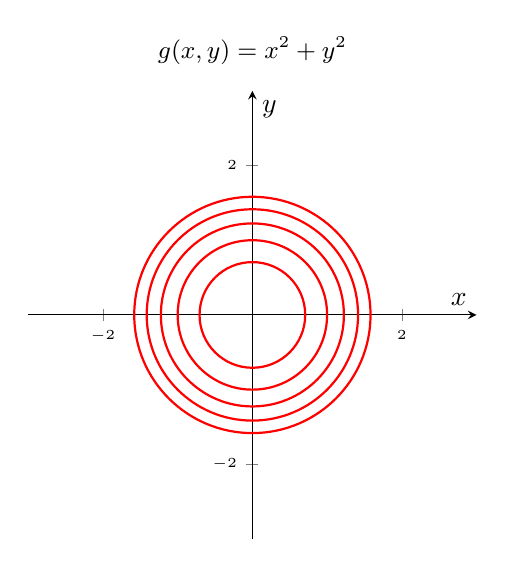
\begin{tikzpicture}
\begin{axis}[
    title={$g(x,y)=x^2+y^2$},
    xlabel=$x$, ylabel=$y$,
    xmin=-3, xmax=3, ymin=-3, ymax=3,
    axis lines=middle,
    axis equal image,
    tick label style={font=\tiny},
    title style={font=\small}
]
    \pgfplotsinvokeforeach{0.5, 1.0, 1.5, 2.0, 2.5}{
        \draw[red, thick] (axis cs:0,0) circle [radius={sqrt(#1)}];
    }
\end{axis}
\end{tikzpicture}
\end{minipage}
\hfill
\begin{minipage}[t]{0.32\textwidth}
\centering
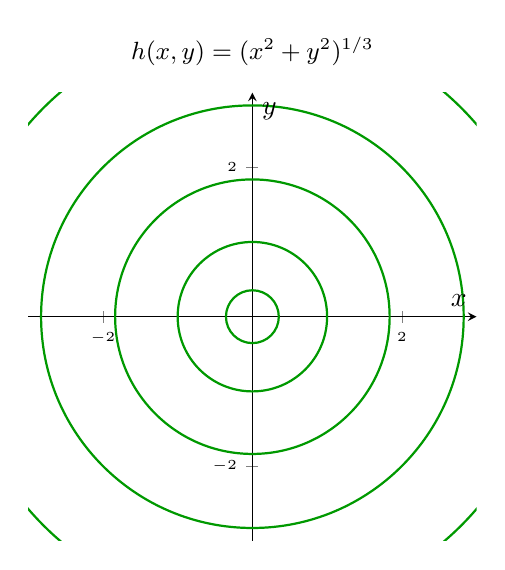
\begin{tikzpicture}
\begin{axis}[
    title={$h(x,y)=(x^2+y^2)^{1/3}$},
    xlabel=$x$, ylabel=$y$,
    xmin=-3, xmax=3, ymin=-3, ymax=3,
    axis lines=middle,
    axis equal image,
    tick label style={font=\tiny},
    title style={font=\small}
]
    \pgfplotsinvokeforeach{0.5, 1.0, 1.5, 2.0, 2.5}{
        \draw[green!60!black, thick] (axis cs:0,0) circle [radius={#1^(1.5)}];
    }
\end{axis}
\end{tikzpicture}
\end{minipage}
\end{figure}

\subsection{Visualizing Higher Dimensions via Slices}

\begin{itemize}
    \item A sphere in $\mathbb{R}^3$ defined by $x^2 + y^2 + z^2 = \rho^2$ can be sliced along $z = c$ to produce 2D circular cross-sections in $\mathbb{R}^2$.
    \item A 3-sphere in $\mathbb{R}^4$ defined by $x^2 + y^2 + z^2 + w^2 = R^2$ can be visualized through its 3D cross-sections ($w = c$), which appear as concentric 2-spheres in $\mathbb{R}^3$ whose radii expand from $0$ to $R$ and then contract back to $0$.
\end{itemize}

\begin{figure}[htbp]
\centering
% 3D Sphere Slices
\begin{minipage}[t]{0.48\textwidth}
\centering
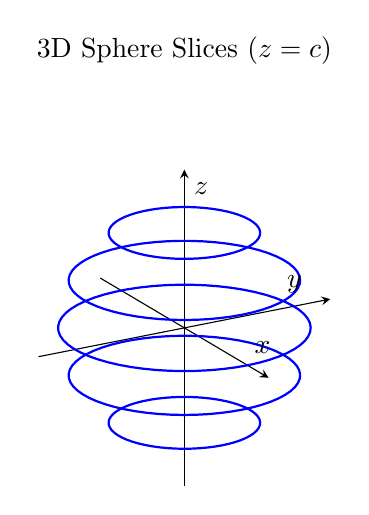
\begin{tikzpicture}
\begin{axis}[
    view={60}{20},
    axis lines=center,
    xlabel=$x$, ylabel=$y$, zlabel=$z$,
    xmin=-2, xmax=2, ymin=-2, ymax=2, zmin=-2, zmax=2,
    ticks=none,
    unit vector ratio=1 1 1,
    scale=1.2,
    title={3D Sphere Slices ($z = c$)},
]
    \pgfplotsinvokeforeach{-1.2, -0.6, 0, 0.6, 1.2}{
        \pgfmathsetmacro{\r}{sqrt(2.25 - (#1)^2)}
        \addplot3[domain=0:360, samples=60, blue, thick] ({\r*cos(x)}, {\r*sin(x)}, {#1});
    }
\end{axis}
\end{tikzpicture}
\end{minipage}
\hfill
% 4D Hypersphere Slices in 3D (3D Spheres with varying radii)
\begin{minipage}[t]{0.48\textwidth}
\centering
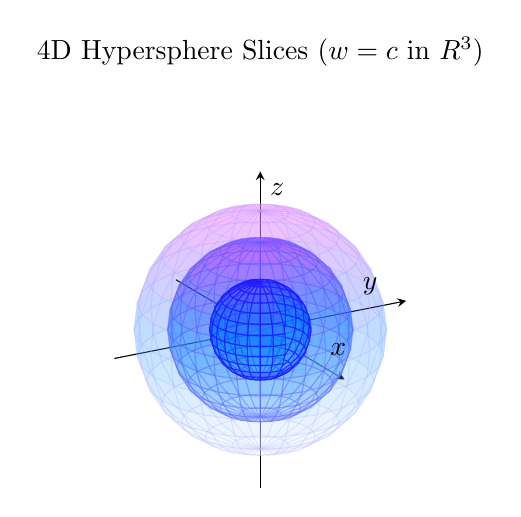
\begin{tikzpicture}
\begin{axis}[
    view={60}{20},
    axis lines=center,
    xlabel=$x$, ylabel=$y$, zlabel=$z$,
    xmin=-2, xmax=2, ymin=-2, ymax=2, zmin=-2, zmax=2,
    ticks=none,
    unit vector ratio=1 1 1,
    title={4D Hypersphere Slices ($w = c$ in $\mathbb{R}^3$)},
    scale=1.2,
]
    \addplot3[
        surf, domain=0:180, domain y=0:360, samples=15, samples y=25,
        colormap/cool, opacity=0.15, faceted color=blue!30
    ] ({1.5*sin(x)*cos(y)}, {1.5*sin(x)*sin(y)}, {1.5*cos(x)});

    \addplot3[
        surf, domain=0:180, domain y=0:360, samples=15, samples y=25,
        colormap/cool, opacity=0.35, faceted color=blue!60
    ] ({1.1*sin(x)*cos(y)}, {1.1*sin(x)*sin(y)}, {1.1*cos(x)});

    \addplot3[
        surf, domain=0:180, domain y=0:360, samples=15, samples y=25,
        colormap/cool, opacity=0.65, faceted color=blue!90
    ] ({0.6*sin(x)*cos(y)}, {0.6*sin(x)*sin(y)}, {0.6*cos(x)});

\end{axis}
\end{tikzpicture}
\end{minipage}
\end{figure}